\begin{figure}[htbp]
\centering
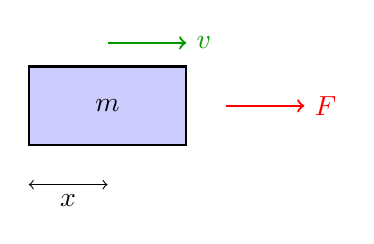
\begin{tikzpicture}
    % Mass
    \draw[thick, fill=blue!20] (0,0) rectangle (2,1);
    \node at (1,0.5) {$m$};

    % Force arrow
    \draw[->, thick, red] (2.5,0.5) -- (3.5,0.5) node[right] {$F$};

    % Velocity arrow
    \draw[->, thick, green!60!black] (1,1.3) -- (2,1.3) node[right] {$v$};

    % Position reference
    \draw[<->] (0,-0.5) -- (1,-0.5) node[midway, below] {$x$};
\end{tikzpicture}
\caption{Mass element with applied force, coordinate system, and ground reference.}
\label{fig:mass_element}
\end{figure}
